\chapter{System Architecture}
%Welche Teilprobleme leiten sich aus der Zielstellung weiter ab?
%Was sind die Rahmenbedingungen für die Probleme und wie können wir diese lösen.
%
%Lösungsbeschreibung, warum so?
%
%Bauen Sie auf der Methodik aus der Einführung auf.
%Ein System bauen und dann beobachten (machen Sie wohl meistens)
%
%z.B. wenn Sie ein System bauen. Wie sieht Ihre Architektur aus? Was sind die Resultate des
%Entwurfs? Welche Alternativen gibt es zu Ihrem Entwurf? Warum haben Sie sich gerade für
%Ihre Lösung entschieden? Was sind deren Vor­ und Nachteile?
%
%Welche Prozesse unterstützt die Architektur?
%Datenquellen?
%Transformationen?
%Datenverarbeitung?

TODO:
Distributed system -> distributed collection with clients, software solution is a streaming platform itself,
cloud environments, client server architecture, client-management with service-discovery, explain", communication via REST,
Publish(client) -> Topic <- Subscribe Logstash,

continuous, distributed, time-series "data feed", difference raw and aggregated\cite{Klepp16},
events as "immutable facts", why? explain data samples (cpu, disk...)
state state of system at time, on host, at port, the type of collector and data.

arch uses both, raw because of unknown data consumers, flink-job-index for demonstration
of SP.

Pipeline: Collect-Transport-Persistence, see \cite{VanL14}

\begin{figure}[H]
	\centering
	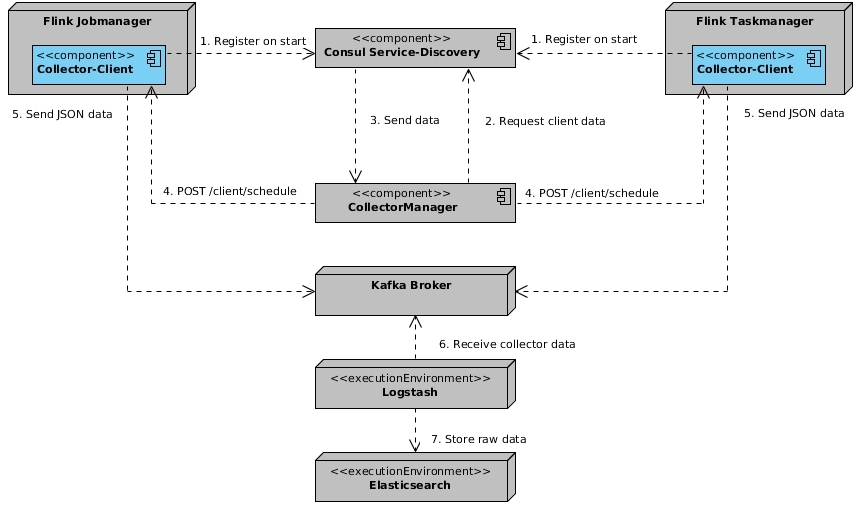
\includegraphics[width=1.0\textwidth]{../uml/component-diagram.jpg}
	\caption{Component diagram}
	\label{component-diagram}
\end{figure}

\section{CollectorClient}

The CollectorClient tier is our entry point for bringing data into the system , module to gather the data streams
from data sources, installed on source systems, a small service that needs to be installed on source systems

data layer

\begin{figure}[H]
	\centering
	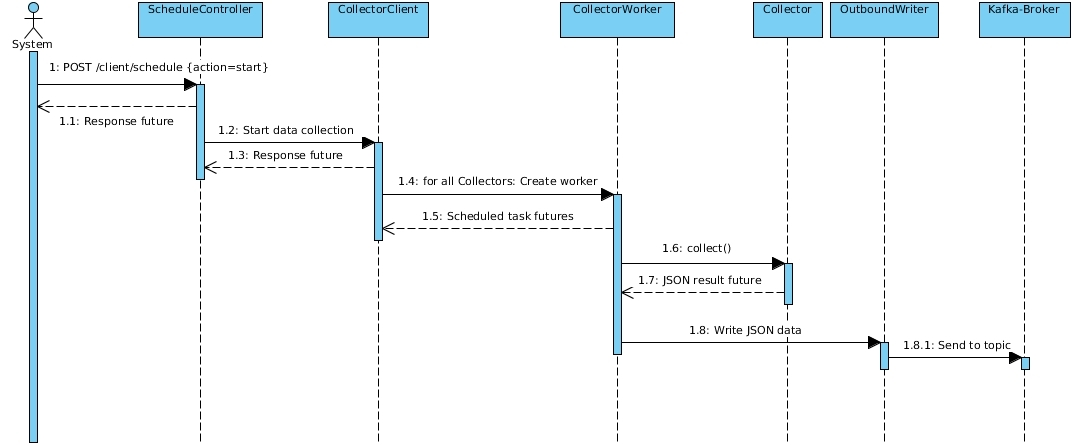
\includegraphics[width=1.0\textwidth]{../uml/sequence-scheduling.jpg}
	\caption{Sequence diagram 'Client scheduling'}
	\label{sequence-diagram-client-scheduling}
\end{figure}

\section{CollectorManager}

Clients need to be scheduled -> management component for Collector clients, gives overview and enables start/stop of
registred CollectorClients, uses Consulas client-discovery backend, why? First experiments with implementing a "client-registry",
heartbeats, needed another db for storing clients, Consul because of registry for components in distributed systems

\begin{figure}[H]
	\centering
	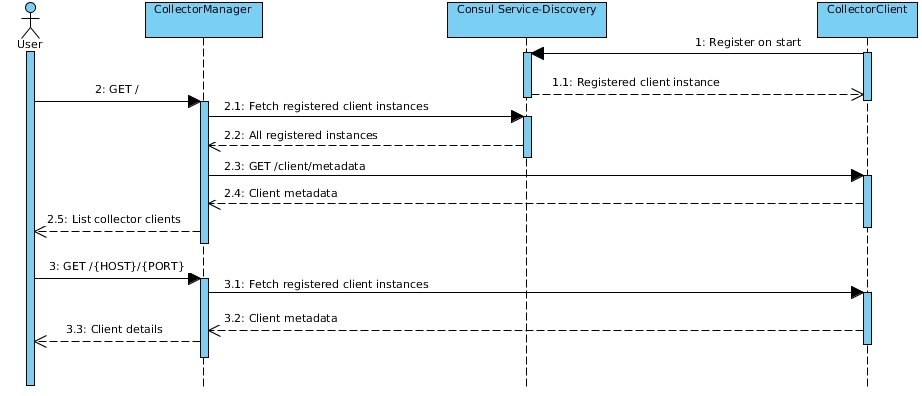
\includegraphics[width=1.0\textwidth]{../uml/sequence-discovery.jpg}
	\caption{Sequence diagram 'Client discovery'}
	\label{sequence-diagram-client-discovery}
\end{figure}

%\section{Client-Discovery}
%
%Registration for CollectorClients
\section{Message-Broker}

The Message-Broker integrates distributed collector-client to an overall system by providing a
message queue for transmitting data between them. The CollectorClients can publish
its data to the queue and the other applications can asynchronously read it from the queue at any time.
Message Broker systems persist incoming messages in an special type of a message queue, named topic.

Queueing, see Marz15, compute layer
Transport, "Event-Log", see \cite{Kreps13}
Collect the streams and make them available for consumption

\section{Indexer}

Receive messages from Message-Broker, route data, create ES index, why, describe context BDAA, compute layer

\section{Persistence}

ES as search index for time-series based data, easy visualization with Kibana, why?, searchable, common in BDA, storage layer

\section{Technologies}

The following section introduces the infrastructure components used to realize the software architecture described above.

\begin{itemize}
%	\item Spring-Boot  WHY
%	\item Spring-Kafka  WHY
%	\item Eclipse Jetty servlet container  WHY
	\item Apache Kafka message broker  WHY
	\item Logstash indexer  WHY
	\item Elasticsearch search index  WHY
\end{itemize}

\section{Summary}

Summarize architecture, discuss benefits and disadvantages.

%READ
%Messaging is the art of moving message across the producer and consumer
%group. It integrates distributed applications to an overall system by providing
%message queues for communication between them. One application can publish
%its messages to the queue and the other application can asynchronously read it
%from the queue at any time. Message Broker systems persist incoming
%messages in an enhanced type of a message queue, named topic. Sending
%messages to the broker in the form of publishing to a specific topic and on the
%other hand receiving messages only for the specified topic, is called publish /
%subscribe and this therefore classifies Kafka as a publish subscribe system.

%3.3 What is a Topic in Kafka?
%Kafka provides a high-level abstraction called Topic. Users define a new Topic
%(file) for each new category of messages (documents) and the messages are
%published to a category or stream name. A topic allows the message broker to
%deliver messages to multiple independent consumers.
%Kafka has a very simple storage layout. Each partition of a topic (file)
%corresponds to a logical log. Each time a producer publishes a message to a
%topic, the broker appends the message to the last segment file. The message is
%exposed to the consumers after it is flushed.
%
%3.4 Who are Producers in Kafka?
%Producers are the clients publishing messages to a Topic. Producers are diverse
%in nature and publish varied messages to different topics. A producer can
%publish data to a topic of its choice and is responsible for choosing which
%message will be assigned to which partition within a topic. Kafka producer client
%is configured to send messages in either a synchronous or asynchronous
%fashion to the topics. The asynchronous mode allows the client to batch small
%messages into larger data chunks before sending them over the network.
%
%3.5 What is a Message Broker?
%A Message Broker is a key element of the solution. It is a dedicated component
%which decouples the source and target systems by assuming full responsibility
%for coordinating communication between all the connected nodes. The
%published messages are stored at a set of servers called Brokers. Each Kafka
%cluster consists of one or more Brokers. The partitions of a Topic are distributed
%over the Brokers of the Kafka cluster with each Broker handling data and
%requests for a share of the partitions. Each partition is replicated across a
%configurable number of Brokers for fault tolerance. The main tasks of a message
%broker are the dynamic registration of endpoints, determining the location of a
%target system, and performing the communication as well as the transformation
%of a message from one format to another.
%A consumer can subscribe to one or more topics from the brokers and consume
%the subscribed messages by pulling data from the Brokers. The Broker locates
%the requested message by searching the list and sends the data back to the
%consumer. After a consumer receives a message it computes the location of the
%next message to consume and uses it in the next pull request.
%
%3.6 Who are Consumers in Kafka?
%The term consumer describes the clients that consume messages from a Topic.
%Producers and Consumers can simultaneously write to and read from multiple
%topics. A consumer always consumes messages from a particular partition
%sequentially. If the consumer acknowledges a particular message it implies that
%the consumer has received all the messages prior to that message. This leads to
%the fact that Kafka relies on the pull-model to reach maximum performance on
%the consumption side.
%Apache Kafka does not keep track of what messages have been consumed on
%the Broker and therefore does not rely on any acknowledgments from the
%consumer. Instead, the position of a consumer is just a single integer on a
%partition which defines the offset of the next message to consume. As a side
%benefit, it permits the consumer to rewind back to an old offset and re-consume
%data. Each consumer is represented as a process and these processes are
%organized within groups called consumer groups as Kafka supports the concept
%of consumer groups. Each consumer group consists of one or more consumers
%that jointly consume a set of subscribed topics.



